\documentclass[11pt]{article}

\title{Multiple Regression Techniques and Unsupervised Learning for Predicting Urban Land Covers}
\author{Jonas Wallstein and Joshua Chen}
\usepackage{amsmath}
\usepackage{amssymb}
\usepackage{url}
\usepackage{hyperref}
\usepackage{graphicx}
\usepackage{xcolor}
\usepackage{subcaption}
\usepackage{booktabs} 



% Set default color for table of contents entries
\renewcommand{\contentsdefaultcolor}{\color{black}}

% Hyperref setup for clickable links in the PDF
\usepackage{hyperref}
\hypersetup{
    colorlinks=true,
    linkcolor=black,
    urlcolor=black,
    citecolor=black
}
\usepackage[margin=1in]{geometry}
\date{\today} 

\begin{document}
\setlength{\parindent}{0pt}
\maketitle

\tableofcontents

\newpage
\section{Introduction}
The way in which the surface of a city is distributed has a huge impact on human life in the city. Cities with a large share of impervious surfaces have higher risk of floods as water cannot sink into the soil (Feng et al. 2021), and temperatures are more extreme (Kalnay and Cai, 2003). An important aspect for public policy is therefore knowing how the area in a city is distributed. This is especially important in light of the climate crisis which will increase the frequency and severity of extreme weather events such as floods and high temperature.
The distribution of surfaces is referred to as the land cover and is defined as “the composition and characteristics of land surface elements” (Cihlar, 2000). The land cover in an urban area typically includes objects such as asphalt cars and trees. Classification of these objects is vital to assess the share of impervious surfaces in a city and is typically determined by analyzing aerial images. Thus, our outcome variable is the class of an object, which can be one of nine types of urban land cover, for example trees or buildings. The input variables are measures from an aerial image such as the brightness, color or shape of an object. The input data is preprocessed from the pixel level to different “segments”, which are explained in the data section.\\

The goal of this thesis is to classify the urban land cover objects in a setting with a high dimensional feature space. Thus, we use logistic and multinomial regressions with LASSO and Bayesian model selection. Further, we assess the performance of different clustering methods in differentiating the actual number of clusters that correspond to our nine types of land cover. This thesis proceeds with a summary of related work and the data used. Then we use regression and unsupervised learning and finally discuss our methodology and findings.

\section{Related Works}
Urban land cover classification has been primarily done using machine learning methods such as Support Vector Machines (Johnson, 2013), Extreme Gradient Boosting (Georganos, 2018) and in recent years increasingly Deep Learning Models (Zhang et al., 2018; Helber et al., 2019). The latter can be considered state of the art for land cover classification. While such models typically produce better predictions than our regression framework, they lack any availability for interpretability. An approach similar to ours is done using multinomial logistic regression to classify soil depth in Taiwan by Chan et al. (2019).

\section{Dataset}

\subsection{Overview:}
The dataset utilized for the project was found on the UCI Machine Learning Repository. This dataset was donated by Dr. Brian Johnson on March 26th, 2014. Dr. Johnson, a deputy director at the Institute for Global Environmental Strategies, whose projects include mapping urban land covers. This repository contains data from high resolution aerial imagery for classification into nine types of urban land covers with the purpose of  “assist[ing]  sustainable urban planning efforts”.\\

The data provided is already split into a training and testing set. The testing set was created by random sampling. The designated testing set contains 507 samples and the designated training set contains 168 samples. Because the split is arbitrary, the roles of the training set and testing set were switched to have more data for the models to train on. This results in a $75.11\%$, $24.89\%$ train-test split.\\

The dataset contains no missing values.\\

The chart on the right contains the breakdown of the training set and testing set by classification as well as further exploratory variables. As will be discussed later in the paper, immediately the issue of class imbalance becomes readily apparent. 

\begin{table}[h!]
\centering
\begin{tabular}{lcccc}
\hline
& Training & Testing & \% Train Set & \% of Class \\ 
\hline
Asphalt & 45 & 14 & 8.88 & 76.27 \\ 
Trees & 89 & 17 & 17.55 & 83.97 \\ 
Grass & 83 & 29 & 16.37 & 74.11 \\ 
Soil & 20 & 14 & 3.94 & 58.82 \\ 
Concrete & 93 & 23 & 18.34 & 80.17 \\ 
Buildings & 97 & 25 & 19.13 & 79.51 \\ 
Cars & 21 & 15 & 4.14 & 58.33 \\ 
Pool & 14 & 15 & 2.76 & 48.28 \\ 
Shadows & 45 & 16 & 8.88 & 73.77 \\
\hline
\end{tabular}
\caption{Breakdown of Data by Class}
\label{your-label}
\end{table}

\subsection{Features:}
This data comes with a significant amount of preprocessing already. The high resolution aerial imaging has already been converted from pixels to 148 interpretable features. Each feature is repeated seven times - each reflecting a different resolution. The features capture objects’ shape, spectral (color), and size. Area is measured in square meters but the spectral and size are broken down into many elements.\\

Below is the feature legend for the dataset. Suffixes 40, 60, 80, 100, 120, 140 are references to the aforementioned resolution. The descriptions and legend are pulled from the UCI website.

\begin{table}[h]
\centering
\begin{tabular}{|c|c|}
\hline
\textbf{Variable} & \textbf{Description} \\
\hline
\texttt{Class} & Land cover class (nominal) \\
\texttt{BrdIndx} & Border Index (shape variable) \\
\texttt{Area} & Area in m\textsuperscript{2} (size variable) \\
\texttt{Round} & Roundness (shape variable) \\
\texttt{Bright} & Brightness (spectral variable) \\
\texttt{Compact} & Compactness (shape variable) \\
\texttt{ShpIndx} & Shape Index (shape variable) \\
\texttt{Mean\_G} & Green (spectral variable) \\
\texttt{Mean\_R} & Red (spectral variable) \\
\texttt{Mean\_NIR} & Near Infrared (spectral variable) \\
\texttt{SD\_G} & Standard deviation of Green (texture variable) \\
\texttt{SD\_R} & Standard deviation of Red (texture variable) \\
\texttt{SD\_NIR} & Standard deviation of Near Infrared (texture variable) \\
\texttt{LW} & Length/Width (shape variable) \\
\texttt{GLCM1} & Gray-Level Co-occurrence Matrix (texture variable) \\
\texttt{Rect} & Rectangularity (shape variable) \\
\texttt{GLCM2} & Another Gray-Level Co-occurrence Matrix attribute (texture variable) \\
\texttt{Dens} & Density (shape variable) \\
\texttt{Assym} & Assymetry (shape variable) \\
\texttt{NDVI} & Normalized Difference Vegetation Index (spectral variable) \\
\texttt{BordLngth} & Border Length (shape variable) \\
\texttt{GLCM3} & Another Gray-Level Co-occurrence Matrix attribute (texture variable) \\
\hline
\end{tabular}
\caption{Description of Variables}
\label{tab:variables}
\end{table}

\newpage
\section{Regression}
This multi-class regression problem has a heavy emphasis on model selection as very apparent in the ordinary logistic regression section. In his paper, Dr. Brian Johnson addressed this through a blended model, averaging the scores of models trained on the segmented levels of resolution. This seems particularly advantageous towards reducing the high correlation that inevitably arises between corresponding features - such as all the mean values of green. However, for our model selection strategies, we decided to utilize LASSO-BIC, 20-fold LASSO, and Bayesian Model Averaging. As our goal here is purely prediction, explainability and interpretability are secondary concerns.\\

We considered numerous metrics to assess model performance. Our first consideration was overall accuracy across all classes. However, we also considered application cases where false positives or false positives are particularly egregious. Therefore, we also considered precision, recall, and F1 across each class.

\subsection{One vs Rest Regression:}
For multi-class classification, we started with an One-vs-Rest approach towards the multi-classification problem. For each class, a model was fitted to create binary classification on predicting for the respective class. For each test sample, all nine models were utilized to predict  on it. The highest probability across the nine predictions was then selected as the classification. 

\subsubsection{Ordinary Logistic Regression:}
The first method utilized was with simple logistic regression. The results are seen in the figures above.\\

\begin{figure}
    \centering
    \begin{tabular}{p{1.5cm} p{1cm} p{1cm} p{1cm} p{1.3cm} p{1cm} p{1 cm} p{1cm} p{1cm} p{1cm}}
      \toprule
      & Asphalt & Building & Car & Concrete & Grass & Pool & Shadow & Soil & Tree \\
      \midrule
      Asphalt & 13 & 0 & 1 & 1 & 0 & 6 & 1 & 0 & 0 \\
      Building & 0 & 22 & 1 & 7 & 0 & 2 & 2 & 2 & 0 \\
      Car & 0 & 0 & 12 & 1 & 0 & 1 & 0 & 1 & 0 \\
      Concrete & 0 & 2 & 0 & 11 & 0 & 1 & 1 & 3 & 1 \\
      Grass & 0 & 1 & 0 & 0 & 22 & 0 & 1 & 3 & 10 \\
      Pool & 0 & 0 & 0 & 0 & 0 & 5 & 0 & 0 & 0 \\
      Shadow & 1 & 0 & 0 & 0 & 2 & 0 & 11 & 0 & 0 \\
      Soil & 0 & 0 & 1 & 0 & 0 & 0 & 0 & 5 & 0 \\
      Tree & 0 & 0 & 0 & 0 & 1 & 0 & 0 & 0 & 6 \\
      \bottomrule
    \end{tabular}
    \caption{Confusion Matrix for Logistic Regression \\ Overall Accuracy: 0.637 - (0.5593, 0.7096)}
    \label{tab:confusion_matrix}
    \end{figure}%
 
\begin{figure}
  \centering
  \begin{tabular}{lcccccccccc}
    \toprule
    Metric & Asphalt & Building & Car & Concrete & Grass & Pool & Shadow & Soil & Tree & Average \\
    \midrule
    Precision & 0.565 & 0.579 & 0.800 & 0.550 & 0.564 & 1.00 & 0.786 & 0.714 & 0.857 & 0.713\\
    Recall & 0.929 & 0.880 & 0.800 & 0.478 & 0.759 & 0.333 & 0.688 & 0.357 & 0.353 & 0.620\\
    F1 & 0.703 & 0.698 & 0.800 & 0.512 & 0.647 & 0.500 & 0.733 & 0.476 & 0.500 & 0.619\\
    \bottomrule
  \end{tabular}
  \caption{Precision, Recall, and F1 Scores for Logistic Regression}
  \label{tab:precision_recall_f1_transposed}
\end{figure}

This has an overall accuracy of 0.6369 with a 95\% confidence interval of (0.5593, 0.7096). Precision, a better metric for indicator of model performance in this unbalanced dataset, indicates poor performance at classification.\\

Furthermore, glm.fit in R, used for the logistic regressions, returned the warning: “... algorithm did not converge… fitted probabilities numerically 0 or 1 occurred”. This indicates extreme overfitting and, quickly predicting on in-sample data indicates this to be the case. Quickly predicting in-sample data returns perfect predictions (1.000 accuracy).\\

\subsubsection{Lasso AIC:}
Our first step for addressing this issue was using LASSO BIC and EBIC as a strong model selection tool. However, as typical, AIC was found to be a much more effective metric for purely prediction. We modified the formula from the BIC function (provided to us in seminar one) to produce our AIC OvR models and predictions on the testing set resulted in an overall accuracy of 0.7976 with 95\% CI of (0.7288,.8556)\\

\begin{figure}
  \centering
  \begin{tabular}{lcccccccccc}
    \toprule
    Metric & Asphalt & Building & Car & Concrete & Grass & Pool & Shadow & Soil & Tree & Average\\
    \midrule
    Precision & 0.867 & 0.657 & 0.933 & 0.833 & 0.676 & 1.000 & 0.938 & 0.818 & 0.900 & 0.847\\
    Recall & 0.929 & 0.920 & 0.933 & 0.652 & 0.862 & 0.733 & 0.938 & 0.643 & 0.529 & 0.793 \\
    F1 & 0.897 & 0.767 & 0.933 & 0.732 & 0.758 & 0.846 & 0.938 & 0.720 & 0.667 & 0.806\\
    \bottomrule
  \end{tabular}
  \caption{Precision, Recall, and F1 Scoresfor LASSO-AIC}
  \label{tab:precision_recall_f1_averages}
\end{figure}
 
There is clear improvement in performance from simple logistic regression. However, the in-sample prediction was at near-perfect 99.41\%, still indicating there to be a significant amount of overfitting. Apparently there is still much room for improvement.

\subsubsection{20-Fold Lasso:}
With clear room for improvement, we tried LASSO again - this time set by 20 fold cross validation. We see a significant jump in performance across all metrics (see figure 4). Overall accuracy jumped to 0.8393 with 95\% CI (0.7749, 0.8913).

\begin{figure}
  \centering
  \begin{tabular}{lcccccccccc}
    \toprule
    Metric & Asphalt & Building & Car & Concrete & Grass & Pool & Shadow & Soil & Tree & Average \\
    \midrule
    Precision & 1.000 & 0.733 & 0.933 & 0.667 & 0.806 & 1.000 & 0.941 & 1.000 & 0.875 & 0.884 \\
    Recall & 0.929 & 0.880 & 0.933 & 0.783 & 0.862 & 1.000 & 1.000 & 0.286 & 0.824 & 0.833 \\
    F1 & 0.963 & 0.800 & 0.933 & 0.720 & 0.833 & 1.000 & 0.970 & 0.444 & 0.848 & 0.835 \\
    \bottomrule
  \end{tabular}
  \caption{Precision, Recall, and F1 Scores for LASSO-CV}
  \label{tab:precision_recall_f1_transposed}
\end{figure}

\subsubsection{Bayesian Model Averaging:}

Finally, we employed Bayesian Model Averaging. With the conservative assumption that we do not have good prior knowledge, we chose a Zellner’s prior with g=1. We then chose Beta-Binomial(1,1) as our prior on $\gamma$. Clearly, from the metrics as seen in figure 5, this was by far the best predictor. The overall average from this model was 0.8571 with 95\% CI (0.7949, 0.9063). \\

While Bayesian Model Averaging produced the best results, it was far too computationally expensive relative to the other models. For reference, to train 9 models and predict both testing and in-sample data took LASSO-AIC an elapsed time of 1.86 seconds and LASSO-CV an elapsed time of 31.80 seconds. To train the singular model for predicting "Asphalt" using BMA  took an elapsed time of 581.33 seconds. Training all 9 models would often take upwards of 100 minutes.

\begin{figure}
  \centering
  \begin{tabular}{lcccccccccc}
    \toprule
    Metric & Asphalt & Building & Car & Concrete & Grass & Pool & Shadow & Soil & Tree & Average \\
    \midrule
    Precision & 1.000 & 0.733 & 0.933 & 0.667 & 0.806 & 1.000 & 0.941 & 1.000 & 0.875 & 0.892 \\
    Recall & 0.929 & 0.880 & 0.933 & 0.783 & 0.862 & 1.000 & 1.000 & 0.286 & 0.824 & 0.852 \\
    F1 & 0.963 & 0.800 & 0.933 & 0.720 & 0.833 & 1.000 & 0.970 & 0.444 & 0.848 & 0.858 \\
    \bottomrule
  \end{tabular}
  \caption{Precision, Recall, and F1 Scores for BMA}
  \label{tab:precision_recall_f1_transposed}
\end{figure}

\subsection{One vs. One}
To juxtapose our one vs rest models so far, we implemented a one vs one approach using LASSO-CV.  As this approach requires 36 models, BMA would be far too computationally expensive and LASSO-CV has already proven to be similarly effective. Each model will then output one of the two predictions. The final prediction will be the majority agreement of the predictors. \\

\begin{figure}
    \centering
    \begin{tabular}{p{1.5cm} p{1.1cm} p{1.2cm} p{1cm} p{1.3cm} p{1cm} p{1 cm} p{1cm} p{1cm} p{1cm}}
      \toprule
      & Asphalt & Building & Car & Concrete & Grass & Pool & Shadow & Soil & Tree \\
      \midrule
      Asphalt & 14 & 1 & 1 & 0 & 0 & 5 & 1 & 0 & 0 \\
      Building & 0 & 23 & 4 & 5 & 0 & 9 & 0 & 6 & 0 \\
      Car & 0 & 0 & 10 & 0 & 0 & 1 & 0 & 0 & 0 \\
      Concrete & 0 & 1 & 0 & 17 & 0 & 0 & 0 & 2 & 1 \\
      Grass & 0 & 0 & 0 & 0 & 26 & 0 & 0 & 2 & 1 \\
      Pool & 0 & 0 & 0 & 0 & 0 & 0 & 0 & 0 & 0 \\
      Shadow & 0 & 0 & 0 & 0 & 0 & 0 & 15 & 0 & 0 \\
      Soil & 0 & 0 & 0 & 1 & 0 & 0 & 0 & 4 & 0 \\
      Tree & 0 & 0 & 0 & 0 & 3 & 0 & 0 & 0 & 15 \\
      \bottomrule
    \end{tabular}
    \caption{Confusion Matrix for OvO with LASSO-CV \\ Overall Accuracy: 0.7381 - (0.6648, 0.8028)}
    \label{tab:confusion_matrix}
\end{figure}%

One problem with this methodology is its inability to decide between ties. In R, this will, by default, go to the earlier class. For example, if there are 7 models that predict ‘car’ and 7 that predict ‘grass’, the final prediction would be ‘car’. This is clearly an issue as seen in the confusion matrix. I did remove all 14 instances with ties from the predictions. While this did boost the accuracy to 0.7922 with a 95\% CI (0.7195, 0.8533), this is still considerably worse the OvR LASSO-CV.

Surprisingly, while we expected OvO to be better at dealing with class imbalance, it apparently really struggled with pool and soil - two of the smaller classes.

\subsection{SMOTE Oversampling with 20-Fold LASSO CV:}
As touched upon previously, class imbalance can be an issue with multi-class problems. One technique we used to address this issue is with SMOTE oversampling. We once again did a One vs Rest regression using a 20 fold Lasso logistic regression. The number of samples was arbitrarily set 900 to achieve around a 50\% target classification.\\

\begin{figure}
    \centering
  \begin{tabular}{lcccccccccc}
  \toprule
  & Asphalt & Building & Car & Concrete & Grass & Pool & Shadow & Soil & Tree \\
  \midrule
  Asphalt & 13 & 0 & 0 & 0 & 0 & 0 & 1 & 0 & 0 \\
  Building & 0 & 22 & 0 & 6 & 0 & 0 & 0 & 1 & 0 \\
  Car & 0 & 1 & 15 & 0 & 0 & 0 & 0 & 0 & 0 \\
  Concrete & 0 & 0 & 0 & 16 & 1 & 0 & 0 & 1 & 1 \\
  Grass & 0 & 1 & 0 & 0 & 27 & 0 & 0 & 2 & 6 \\
  Pool & 0 & 0 & 0 & 0 & 0 & 14 & 0 & 0 & 0 \\
  Shadow & 1 & 0 & 0 & 0 & 0 & 1 & 15 & 0 & 0 \\
  Soil & 0 & 1 & 0 & 1 & 0 & 0 & 0 & 10 & 0 \\
  Tree & 0 & 0 & 0 & 0 & 1 & 0 & 0 & 0 & 10 \\
  \bottomrule
   \end{tabular}
   \captionsetup{justification=centering}
    \caption{Confusion Matrix for LASSO-CV/OVR/SMOTE Oversampling\\ Overall Accuracy: 0.8452 - (0.7815, 0.8963)}
    \label{tab:confusion_matrix}
\end{figure}%

SMOTE Oversampling performed better with an accuracy of  0.8452 and 95\% CI (0.7815, 0.8963).  The mean precision was marginally worse and the mean recall was marginally better. However, the more important metric is the variance of these metrics.  Precision had a variance of 0.00694, recall is 0.0201641, and F1 is 0.008895928. For LASSO CV: Precision is 0.0153, recall is 0.0475, and F1 is 0.0298. What this represents is that, without Oversampling, LASSO-CV clearly does a good job with some classes and really poorly with others. However, with Oversampling, the ability of the model to predict any class is much more balanced.

\begin{figure}
  \centering
  \begin{tabular}{lcccccccccc}
    \toprule
    Metric & Asphalt & Building & Car & Concrete & Grass & Pool & Shadow & Soil & Tree & Average \\
    \midrule
    Precision & 0.929 & 0.759 & 0.938 & 0.842 & 0.750 & 1.000 & 0.882 & 0.833 & 0.909 & 0.871 \\
    Recall & 0.929 & 0.880 & 1.000 & 0.696 & 0.931 & 0.933 & 0.938 & 0.714 & 0.588 & 0.845 \\
    F1 & 0.929 & 0.815 & 0.968 & 0.762 & 0.831 & 0.966 & 0.909 & 0.769 & 0.714 & 0.851 \\
    \bottomrule
  \end{tabular}
  \caption{Precision, Recall, and F1 Scores for LASSO-CV with SMOTE Oversampling}
  \label{tab:precision_recall_f1_transposed}
\end{figure}

\section{Unsupervised Learning}
\subsection{Overview:}
Our goal in this section is to assess whether different clustering algorithms can detect the various types of urban land cover in the data and correctly form the corresponding clusters. However, clustering methods such as Gaussian Mixture Models (GMM) and K-Means tend to perform poorly in high-dimensional settings – often described as the "curse of dimensionality," a term coined by Bellman (1957). This is because, as the number of dimensions increases, distances between points become less distinct, and the relative distance between any two points tends to converge. Moreover, relevant clusters may exist only within certain feature subspaces.\\
When we attempted to cluster our original high-dimensional dataframe, we encountered these issues. Neither K-means nor GMMs provided a clear delineation of cluster numbers, indicating these algorithms' inability to distinguish between different clusters effectively. Consequently, we proceeded to reduce the data's dimensionality using various methods and compared the results prior to clustering.

\begin{figure}
  \centering
  \includegraphics[width=1\linewidth]{pca.png}
  \label{fig:yourlabel}
\end{figure}

\subsection{Principal Component Analysis:}
A common approach to reduce the dimensionality of data is Principal Component Analysis (PCA). It transforms a set of possibly correlated variables into a smaller number of uncorrelated variables called principal components while retaining the maximum variability of the original data. The first principal component accounts for the greatest possible variance in the data set, with each subsequent component having the highest variance possible under the constraint that it is orthogonal to the preceding components. Plotting the first two principal components, we can observe the general direction in which the different classes differ. However, there is still significant overlap between the classes, which could cause our clustering methods to miss distinctions between the clusters, at least in this two-dimensional representation. Furthermore, PCA may underperform in high-dimensional settings like ours.

\begin{figure}
  \centering
  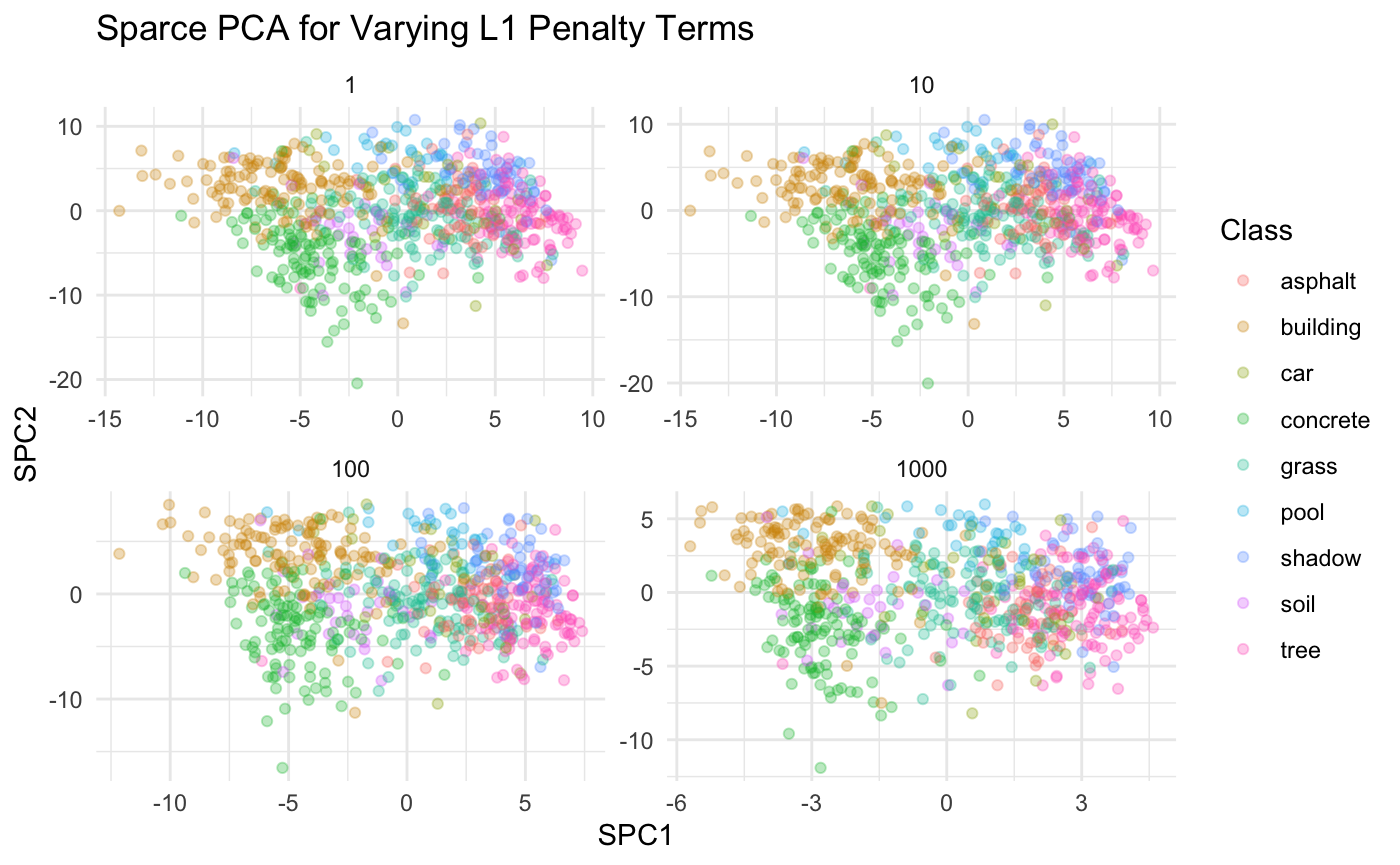
\includegraphics[width=1\linewidth]{Sparce_PCA.png}
  \label{fig:yourlabel}
\end{figure}

\subsection{Sparse Principal Component Analysis}
Our goal with dimensionality reduction is not just to preserve the maximum amount of variance or to minimize the error. Instead, we aim to find a lower-dimensional representation of our data that enhances our ability to discriminate between different types of urban land cover. Therefore, we prioritize identifying principal components that are linear combinations of features crucial for distinguishing between classes, while still preserving as much variance as possible. Unlike standard PCA, which generally utilizes all variables in the dataset to construct each principal component (PC), Sparse PCA constructs PCs from a subset of the original variables. This results in each PC being a linear combination of only a select few variables, achieved through a penalty that enforces sparsity. We employ L1 regularization (similar to Lasso regression), which penalizes the absolute value of the coefficients, introducing sparsity. A penalty strength of 100 has proven effective in separating the clusters in our case, although ideally, this should be confirmed by hyperparameter tuning, such as cross-validation.

\subsection{Contrastive Principal Component Analysis}
Contrastive PCA extends traditional PCA by focusing on identifying patterns that are particularly prominent in a target dataset when contrasted with a background dataset (Abid et al. 2018). The target dataset is expected to contain distinct patterns or features, whereas the background dataset typically represents general, noisy variability. This background data may be similar to the target but lacks the specific features of interest. In our study, the target dataset consists of our actual data, while the background dataset could be represented by random land cover that does not include our nine classes. Due to the absence of a suitable background dataset, we simulated it using two alternative methods.
Firstly, we contrasted features at scales 20 to 60 against those at scales 100 to 140. This approach is based on Johnson's (2013) findings, which indicate that scales 40 to 60 yield the highest classification accuracy, likely because these scales most effectively capture the objects of interest. Conversely, scales 100 to 140, being too coarse, probably represent a mixture of objects and thus can be considered as background data. Secondly, we simulated a background dataset by sampling values from a normal distribution for each column, using the same mean and standard deviation as the corresponding column in the target dataset. However, neither method provided a significant improvement in cluster differentiation over PCA and SPCA. We further investigated whether introducing sparsity, namely applying the sparse contrastive PCA method as outlined by Boileau et al. (2020), would enhance the results, but this too did not lead to better outcomes.

\subsection{Clustering}

Based on the above results, we found PCA and SPCA to be the most promising candidates for dimensionality reduction and proceeded to cluster. Since the SPCA function in R allows a maximum of nine principal components, we chose to use this number for both PCA and SPCA to enable a fair comparison. With K-means clustering, the optimal number of clusters according to the criterion in Tibshirani and Hastie (2001) is 6 for PCA and 3 for SPCA, which are both below the actual 9 classes. Using GMM, the optimal number of clusters is 8 for PCA and 9 for SPCA, very close to the actual number of clusters. However, comparing the number of clusters with the true number of classes is not a sufficient measure of goodness, as the classes are somewhat artificial and depend on explicit choices. For example, the classes asphalt and concrete are very similar and could be combined into one.\\

Since we know the true labels, it is insightful to compare the assigned clusters to those obtained using unsupervised learning. To assess the performance of these assignments, we are using two metrics. The Corrected Rand Index (CRI) is an adjusted measure of similarity between two clusterings, correcting the Rand Index for chance agreement, with a range from -1 (no agreement) to 1 (perfect match). The Variation of Information (VI) index quantifies the amount of information lost or gained between two clusterings, with 0 indicating no difference and higher values indicating less similarity. According to both measures, GMM in combination with SPCA dimension reduction performs the best, achieving a score of 0.47 for CRI and 1.74 for VI. The corresponding clusters are not pure in the sense that they perfectly match the nine classes, but they do detect some patterns. For example, one cluster is almost entirely composed of trees and grass, which are indeed similar.

\subsection{Discussion:}
While we used PCA to reduce dimensionality of our data before clustering, there are more approaches to do clustering in high-dimensionality settings that would have been interesting to explore with more time. While PCA and SPCA globally reduce dimensionality in the dataset, subspace clustering is able to find clusters in different subspaces of a dataset. This would be beneficial for our application as different objects can be identified with different measures. The feature measuring green for example will be more relevant for the trees compared to cars. Further, it would be interesting to investigate how the contrastive PCA methods would perform in this setting with actual background data instead of simulations.

\section{Conclusion}
This project provided us with the opportunity to employ various model selection tools for a multi-class problem. Effectively addressing overfitting was achieved through model selection using Bayesian Model Averaging (BMA) and LASSO-CV. However, due to class imbalance, many models exhibited inconsistency in predicting classes. The application of SMOTE Oversampling successfully mitigated this issue, yielding more consistent results across classes. Moreover, the One vs. Rest approach proved more effective than One vs. One in this scenario.\\

Given more time, several additional methodologies could be explored for their effectiveness. Softmax Regression stands out as a potential solution to eliminate the need for multiple models. Bootstrapping and random oversampling could be alternatives to SMOTE Oversampling. Bayesian Model Averaging, when combined with either SMOTE Oversampling or a One vs. One approach, may yield insightful results with sufficient computational resources.\\

Furthermore, our models operated in a context-independent manner, necessitating the use of F1, Precision, and Recall for evaluation. In hypothetical situations where a false positive carries more significant consequences (emphasizing precision), or when it's preferable to make no prediction rather than an incorrect one, incorporating multiple methods (such as setting a minimum threshold) for probability assessment becomes crucial. Additionally, the paper did not delve into the variables selected by the various methods. \\

Concerning unsupervised learning we investigated different methods for dimensionality reduction including PCA, sparse PCA, contrastive PCA and sparse contrastive PCA. We then used the reduced dimensionality data to find clusters using the K-means clustering and Gaussian Mixture Models. While we used PCA to reduce dimensionality of our data before clustering, there are more approaches to do clustering in high-dimensionality settings that would have been interesting to explore with more time. While PCA and SPCA globally reduce dimensionality in the dataset, subspace clustering methods such as CLIQUE are able to find clusters in different subspaces of a dataset. This would be beneficial for our application as different objects can be identified with different measures. The feature measuring green for example will be more relevant for the trees compared to cars. Further, it would be interesting to investigate how the contrastive PCA methods would perform in this setting with actual background data instead of simulations.

\section{Bibliography}
Abid, A., Zhang, M.J., Bagaria, V.K., Zou, J., 2018. Exploring patterns enriched in a dataset with contrastive principal component analysis. Nat Commun 9, 2134. https://doi.org/10.1038/s41467-018-04608-8\\

Bellman, R., 1966. Dynamic programming. Science, 153(3731), pp.34-37.\\

Boileau, P., Hejazi, N.S., Dudoit, S., 2020. Exploring high-dimensional biological data with sparse contrastive principal component analysis. Bioinformatics 36, 3422–3430. \\https://doi.org/10.1093/bioinformatics/btaa176\\

Chan, H.C., Chang, C.C., Chen, P.A., Lee, J.T., 2019. Using multinomial logistic regression for prediction of soil depth in an area of complex topography in Taiwan. CATENA 176, 419–429. https://doi.org/10.1016/j.catena.2019.01.030\\

Cihlar, J., 2000. Land cover mapping of large areas from satellites: status and research priorities. International journal of remote sensing, 21(6-7), pp.1093-1114.\\
 
Feng, B., Zhang, Y., Bourke, R., 2021. Urbanization impacts on flood risks based on urban growth data and coupled flood models. Nat Hazards 106, 613–627. https://doi.org/10.1007/s11069-020-04480-0\\

Georganos, S., Grippa, T., Vanhuysse, S., Lennert, M., Shimoni, M., Wolff, E., 2018. Very High Resolution Object-Based Land Use–Land Cover Urban Classification Using Extreme Gradient Boosting. IEEE Geosci. Remote Sensing Lett. 15, 607–611. https://doi.org/10.1109/LGRS.2018.2803259\\

Helber, P., Bischke, B., Dengel, A., Borth, D., 2019. EuroSAT: A Novel Dataset and Deep Learning Benchmark for Land Use and Land Cover Classification. IEEE J. Sel. Top. Appl. Earth Observations Remote Sensing 12, 2217–2226. https://doi.org/10.1109/JSTARS.2019.2918242\\

Johnson, B.A., 2013. High-resolution urban land-cover classification using a competitive multi-scale object-based approach. Remote Sensing Letters 4, 131–140. https://doi.org/10.1080/2150704X.2012.705440\\

Kalnay, E., Cai, M., 2003. Impact of urbanization and land-use change on climate. Nature 423, 528–531. https://doi.org/10.1038/nature01675\\

Tibshirani, R., Walther, G., Hastie, T., 2001. Estimating the number of clusters in a data set via the gap statistic. Journal of the Royal Statistical Society: Series B (Statistical Methodology) 63, 411–423. https://doi.org/10.1111/1467-9868.00293\\

Zhang, P., Ke, Y., Zhang, Z., Wang, M., Li, P. and Zhang, S., 2018. Urban land use and land cover classification using novel deep learning models based on high spatial resolution satellite imagery. Sensors, 18(11), p.3717.\\

\section{Appendix}



 
\end{document}